\documentclass[preprint,1p,times]{elsarticle}

\usepackage{booktabs}
\usepackage{hyperref}

\makeatletter
\def\ps@pprintTitle{%
 \let\@oddhead\@empty
 \let\@evenhead\@empty
 \def\@oddfoot{}%
 \let\@evenfoot\@oddfoot}
\makeatother

\usepackage{graphicx}
\usepackage{amssymb}
\usepackage{commath}
\usepackage{mathtools}
\usepackage{subcaption}
\usepackage{float}
\usepackage{lineno}

\linenumbers

\DeclareMathOperator*{\E}{\mathbb{E}}
\graphicspath{ {./graphics/} }

\begin{document}

\begin{frontmatter}

\vspace*{\fill}
\begin{center}
This is a draft version of work in progress, content will be revisited in subsequent versions.
\end{center}
\vspace*{\fill}
    
\title{Robust Local Polynomial Regression with Similarity Kernels}
\author{Yaniv Shulman}
\address{yaniv@shulman.info}


\begin{abstract}
Local polynomial regression is a powerful and flexible statistical technique that has gained increasing popularity in recent years due to its ability to model complex relationships between variables. Local polynomial regression generalizes the polynomial regression and moving average methods by fitting a low-degree polynomial to a nearest neighbors subset of the data at the location. The polynomial is fitted using weighted ordinary least squares, giving more weight to nearby points and less weight to points further away. Local polynomial regression is however susceptible to outliers and high leverage points which may cause an adverse impact on the estimation accuracy. The main contribution of this paper is to revisit the kernel that is used to produce local regression weights. The simple yet effective idea is to generalize the kernel such that both the predictor and the response are used to calculate weights. Within this framework, two positive definite kernels are proposed that assign robust weights to mitigate the adverse effect of outliers in the local neighborhood by estimating and utilizing the density at the local locations. The method is implemented in the Python programming language and is made publicly available at \url{https://github.com/yaniv-shulman/rsklpr}. Experimental results on synthetic benchmarks across a range of settings demonstrate that the proposed method achieves competitive results and generally improves on the standard local polynomial regression method.
\end{abstract}
\end{frontmatter}

\section{Introduction}
\label{s:Introduction}
Local polynomial regression (LPR) is a powerful and flexible statistical technique that has gained increasing popularity in recent years due to its ability to model complex relationships between variables. Local polynomial regression generalizes the polynomial regression and moving average methods by fitting a low-degree polynomial to a nearest neighbors subset of the data at the location. The polynomial is fitted using weighted ordinary least squares, giving more weight to nearby points and less weight to points further away. The value of the regression function for the point is then obtained by evaluating the fitted local polynomial using the predictor variable value for that data point. LPR has good accuracy near the boundary and performs better than all other linear smoothers in a minimax sense \citep{Avery2010LiteratureRF}. The biggest advantage of this class of methods is not requiring a prior specification of a function i.e. a parametrized model. Instead only a small number of hyperparameters need to be specified such as the type of kernel, a smoothing parameter and the degree of the local polynomial. The method is therefore suitable for modeling complex processes such as non-linear relationships, or complex dependencies for which no theoretical models exist. These two advantages, combined with the simplicity of the method, makes it one of the most attractive of the modern regression methods for applications that fit the general framework of least squares regression but have a complex deterministic structure. 

Local polynomial regression incorporates the notion of proximity in two ways. The first is that a smooth function can be reasonably approximated in a local neighborhood by a simple function such as a linear or low order polynomial. The second is the assumption that nearby points carry more importance in the calculation of a simple local approximation or alternatively that closer points are more likely to interact in simpler ways than far away points. This is achieved by a kernel which produces values that diminish as the distance between the explanatory variables increase to model stronger relationship between closer points. 

Methods in the LPR family include the Nadaraya-Watson estimator \citep{Nadaraya1964OnER, Watson1964SmoothRA} and the estimator proposed by Gasser and M{\"u}ller \citep{Gasser1984EstimatingRF} which both perform kernel based local constant fit. These were improved on in terms
of asymptotic bias by the proposal of the local linear and more general local polynomial estimators \citep{Stone1977ConsistentNR, clevland79, 85a168c3-c6d4-3039-8afe-b1944919c518, clevland_devlin88, fan_1993}. For a review of LPR methods the interested reader is referred to \citep{Avery2010LiteratureRF}.

LPR is however susceptible to outliers, high leverage points and functions with discontinuities in their derivative which often cause an adverse impact on the regression due to its use of least squares based optimization \citep{10.1002/wics.1492}. The use of unbounded loss functions may result in anomalous observations severely affecting the local estimate. Substantial work has been done to develop algorithms to apply LPR to difficult data. To alleviate the issue \citep{10.1214/aos/1024691246} employs variable bandwidth to exclude observations for which residuals from the resulting estimator are large. In \citep{clevland79} an iterated weighted fitting procedure is proposed that assigns in each consecutive iteration smaller weights to points that are farther then the fitted values at the previous iteration. The process repeats for a number of iterations and the final values are considered the robust parameters and fitted values. An alternative common approach is to replace the squared prediction loss by one that is more robust to the presence of large residuals by increasing more slowly or a loss that has an upper bound such as the Tukey or Huber loss. These methods however require specifying a threshold parameter for the loss to indicate atypical observations or standardizing the errors using robust estimators of scale \citep{Maronna2006RobustST}. For a recent review of robust LPR and other nonparametric methods see \citep{10.1002/wics.1492, SALIBIANBARRERA2023}

The main contribution of this paper is to revisit the kernel used to produce regression weights. The simple yet effective idea is to generalize the kernel such that both the predictor and the response are used to calculate weights. Within this framework, two positive definite kernels are proposed that assign robust weights to mitigate the adverse effect of outliers in the local neighborhood by estimating the density of the response at the local locations. Note the proposed framework does not preclude the use of robust loss functions, robust bandwidth selectors and standardization techniques. In addition the method is implemented in the Python programming language and is made publicly available. Experimental results on synthetic benchmarks demonstrate that the proposed method achieves competitive results and generally performs better than LOESS/LOWESS using only a single training iteration.

The remainder of the paper is organized as follows: In section \ref{S:Local polynomial regression}, a brief overview of the mathematical formulation of local polynomial regression is provided. In section \ref{S:Robust weights with similarity kernels}, a framework for robust weights as well as specific robust positive definite kernels are proposed. In section \ref{S:Experiments and implementation notes}, implementation notes and experimental results are provided. Finally, in section \ref{S:Future work and research directions}, the paper concludes with directions for future research.

\section{Local polynomial regression}
\label{S:Local polynomial regression}
This section provides a brief overview of local polynomial regression and establishes the notation subsequently used. Let $( X, Y )$ be a random pair and $\mathcal{D}_T = \{(X_i,Y_i)\}_{i=1}^{T} \subseteq \mathcal{D}$ be a training set comprising a sample of $T$ data pairs. Suppose that $(X , Y) \sim f_{XY}$ a continuous density and $X \sim f_X$ the marginal distribution of $X$. Let $Y \in \mathbb{R}$ be a continuous response and assume a model of the form $Y_i=m(X_i) + \epsilon_i, \; i \in 1,... \, ,T$ where $m(\cdot): \mathbb{R}^d \rightarrow \mathbb{R }$ is an unknown function and $\epsilon_i$ are independently distributed error terms having zero mean representing random variability not included in $X_i$ such that $\mathbb{E}[Y \, | \,X=x] = m(x)$. There are no global assumptions about the function $m(\cdot)$ other than that it is smooth and that locally it can be well approximated by a low degree polynomial as per Taylor’s theorem. Local polynomial regression is a class of nonparametric regression methods that estimate the unknown regression function $m(\cdot)$ by combining the classical least squares method with the versatility of non-linear regression. The local $p$-th order Taylor expansion for $x \in \mathbb{R}$ near a point $X_i$ yields:

\begin{align}
m(X_i) \approx \sum_{j=0}^p \frac{m^{(j)}(x)}{j!} (x - X_i)^j \coloneqq \sum_{j=0}^p \gamma_j(x)(x - X_i)^j
\label{taylor_expansion}
\end{align}

To find an estimate $\hat{m}(x)$ of $m(x)$ the low-degree polynomial \eqref{taylor_expansion} is fitted to the $N$ nearest neighbors using weighted least squares such to minimize the empirical loss $\mathcal{L}_{lpr}( \cdot \, ; \mathcal{D}_N , h)$ :

\begin{align}
\mathcal{L}_{lpr}(x; \mathcal{D}_N , h) \coloneqq \sum_{i=1}^N \left(  Y_i - \sum_{j=0}^p \gamma_j (x) (x - X_i)^j \right)^2 K_h(x - X_i)
\label{loss_lpr}
\end{align}


\begin{align}
\hat{\gamma}(x) \coloneqq \min_{\gamma(x)} \mathcal{L}_{lpr}(x; \mathcal{D}_N,h)
\label{beta_hat}
\end{align}

Where $\gamma, \hat{\gamma} \in \mathbb{R}^{p+1}$; $K_h(\cdot)$ is a scaled kernel, $h \in \mathbb{R}_{> 0}$ is the bandwidth parameter and $\mathcal{D}_N \subseteq \mathcal{D}_T$ is the subset of $N$ nearest neighbors of $x$ in the training set where the distance is measured on the predictors only. Having computed $\hat{\gamma}(x)$ the estimate of $\hat{m}(x)$ is taken as $\hat{\gamma}(x)_1$. Note the term kernel carries here the meaning typically used in the context of nonparametric regression i.e. a non-negative real-valued weighting function that is typically symmetric, unimodal at zero, integrable with a unit integral and whose value is non-increasing for the increasing distance between the $X_i$ and $x$. Higher degree polynomials and smaller $N$ generally increase the variance and decrease the bias of the estimator and vice versa \citep{Avery2010LiteratureRF}. For derivation of the local constant and local linear estimators for the multidimensional case see \citep{Garcia-Portugues2023}.

\section{Robust weights with similarity kernels}
\label{S:Robust weights with similarity kernels}
The main idea presented is to generalize the kernel function used in equation \eqref{loss_lpr} to produce robust weights. This is achieved by using a similarity kernel function defined on the data domain $K_{\mathcal{D}}:\mathcal{D}^2 \rightarrow \mathbb{R}_+$ that enables weighting each point and incorporating information on the data in the local neighborhood in relation to the local regression target. 

\begin{align}
\mathcal{L}_{rsk}(x, y; \mathcal{D}_N , H) \coloneqq \sum_{i=1}^N \left(  Y_i - \sum_{j=0}^p \beta_j (x, y) (x - X_i)^j \right)^2 K_{\mathcal{D}} \left((x,y),(X_i, Y_i); H \right)
\label{loss_rsk}
\end{align}

\begin{align}
\hat{\beta}(x,y ; \mathcal{D}_N, H ) \coloneqq \min_{\beta(x,y)} \mathcal{L}_{rsk}(x, y; \mathcal{D}_N , H) 
\label{beta_loss_d}
\end{align}

Where $H$ is the set of bandwidth parameters. There are many possible choices for such a similarity kernel to be defined within this general framework. However, used as a local weighting function, such a kernel should have the following attributes:
\begin{enumerate}
\item Non-negative, $K_{\mathcal{D}}((x,y) , ( x', y') \geq 0$.
\item Symmetry in the inputs, $K_{\mathcal{D}}((x,y) , ( x', y')) = K_{\mathcal{D}}((x', y') , (x,y))$.
\item Tending toward decreasing as the distance in the predictors increases. That is, given  a similarity function on the response $s(\cdot, \cdot): \mathbb{R}^2 \rightarrow \mathbb{R}_+$, if $s(y, y')$ indicates high similarity the weight should decrease as the distance between the predictors grows, $s(y, y') > \alpha \implies       
K_{\mathcal{D}}((x, y) , ( x + u, y')) \geq K_{\mathcal{D}}((x, y) , (x + v, y')) \; \; \forall \: \norm{u} \leq \: \norm{v}$ and some $\alpha \in \mathbb{R}_+$.
\end{enumerate}

In this work two such useful positive definite kernels are proposed. Similarly to the usual kernels used in \eqref{loss_lpr}, these tend to diminish as the distance between the explanatory variables increases to model stronger relationship between closer points. In addition, the weights produced by the kernels also model the "importance" of the pair $(x,y)$. This is useful for example to down-weight outliers to mitigate their adverse effect on the ordinary least square based regression. Formally let $K_{\mathcal{D}}$ be defined as:

\begin{align}
K_{\mathcal{D}} \left((x,y),(x', y') ; H_1, H_2 \right) &= K_1(x,x' ; H_1) K_2 \left((x,y),(x', y') ; H_2 \right)
\label{compound_kernel_def}
\end{align}

Where $K_1: \mathbb{R}^d \times \mathbb{R}^d \rightarrow \mathbb{R}_+$ and $K_2: \mathcal{D}^2 \rightarrow \mathbb{R}_+$ are positive definite kernels and $H_1$, $H_2$ are the sets of bandwidth parameters. The purpose of $K_1$ is to account for the distance between a neighbor to the local regression target and therefore may be chosen as any of the kernel functions that are typically used in equation \eqref{loss_lpr}. The role of $K_2$ is described now in more detail as this is the main idea proposed in this work. Using $K_2$, the method performs robust regression by detecting local outliers in an unsupervised manner and assigns them with lower weights. There are many methods that could be employed to estimate the extent to which a data point is a local outlier however in this work it is estimated in one of the following two ways.

\begin{figure}[h]
\caption{Loss function, assuming a standard quadratic function of the residual, a standard normal density for $K_2$ and excluding the $K_1$ distance kernel scaling.}
\centering
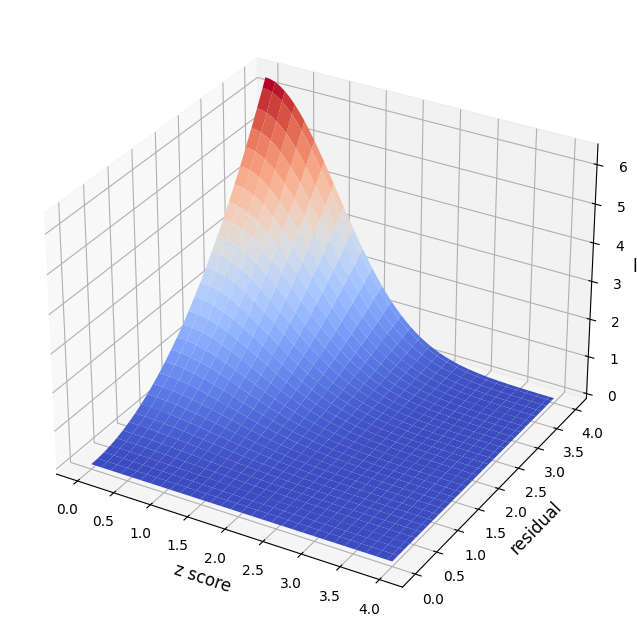
\includegraphics[width=0.5\textwidth]{loss_2d.png}
\end{figure}

\subsection*{Conditional density} 
The first proposed method for $K_2$ is proportional to the estimated localized conditional marginal distribution of the response variable at the location:
\begin{align}
K_2 \left((x,y),(x', y') ; H_2 \right) = \hat{f}(y \, | \, x ; H_2) \hat{f}(y' \, | \, x'; H_2)
\label{cond_kernel_def}
\end{align}
The nonparametric conditional density estimation is performed using the Parzen–Rosenblatt window (kernel density estimator):
\begin{align}
\hat{f}(y \, | \, x; H_2) &= \hat{f} (x, y ; H_2) / \hat{f} (x; H_2) \\
&= \hat{f} (v ; \mathbf{H}_v) / \hat{f} (x; \mathbf{H}_x) \\
&= \frac{|\mathbf{H}_x|^{1/2} \sum_{i=1}^N K_v \left( \mathbf{H}_v^{-1/2} (v - V_i) \right)} {|\mathbf{H}_v|^{1/2} \sum_{i=1}^N K_x \left( \mathbf{H}_x^{-1/2} (x - X_i) \right)}
\label{conditional_prob_est}
\end{align}
Where $v=[x,y] \in \mathbb{R}^{d+1}$ is the concatenated vector of the predictors and the response; and $\mathbf{H}_v, \mathbf{H}_x$ are bandwidth matrices.
\subsection*{Joint density}
The second proposed kernel is proportional to the joint distribution of the random pair, this could be useful for example to also down-weight high leverage points:
\begin{align}
K_2 \left((x,y),(x', y') ; H_2 \right) = \hat{f}(x,y ; H_2) \hat{f}(x',y'; H_2)
\label{joint_kernel_def}
\end{align}
Where the joint density can be estimated using the same aforementioned approach. \newline

Regardless of the choice of kernel, the hyperparameters of this model are similar in essence to the standard local polynomial regression and include the span of included points, the kernels and their associated bandwidths. Note that this estimator can be replaced with a robust alternative and better results are anticipated by doing so however exploring this option is left for future work.

\begin{figure}[t]
\caption{The plot illustrates the proposed loss function, a number of common robust losses and the standard quadratic residual loss for comparison. It is assumed that that $K_2$ is equivalent to the standard normal density and the $K_1$ distance kernel scaling is excluded. The numbers appended to "rsklpr" indicate how many standard deviations away from the mean the density is calculated. It is evident that the loss is heavily attenuated in regions of low density.}
\centering
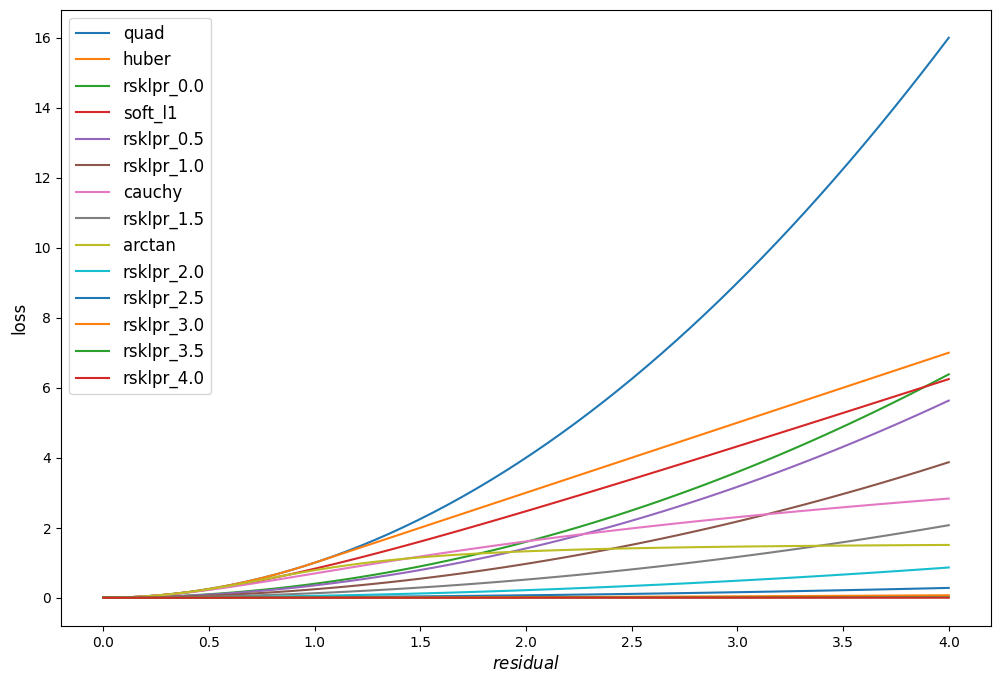
\includegraphics[width=1.0\textwidth]{losses_1d.png}1
\end{figure}

\section{Experiments and implementation notes}
\label{S:Experiments and implementation notes}

\begin{figure}[t]
\caption{Regression example of synthetically generated 1D data with heteroscedastic noise. Additional experimental results and demonstrations including multivariate settings and bootstrap based confidence intervals are available at \url{https://nbviewer.org/github/yaniv-shulman/rsklpr/tree/main/src/experiments/} as interactive Jupyter notebooks \cite{jupyter}}
\centering
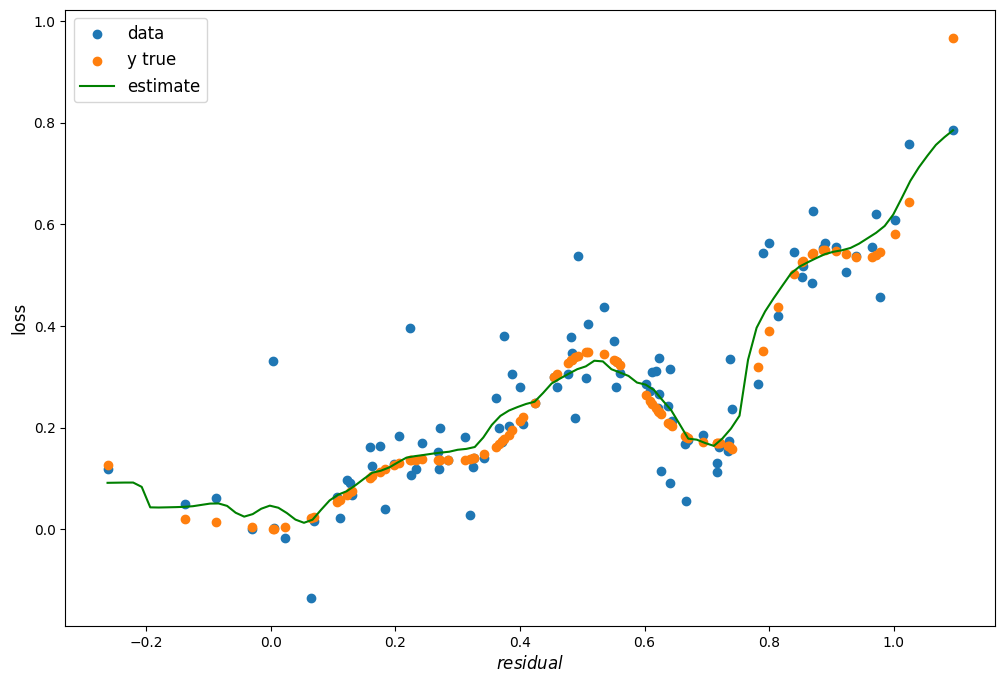
\includegraphics[width=1.0\textwidth]{example_regression_1d_1.png}1
\end{figure}

The proposed method was implemented in Python. The distances between pairs are normalized to the range [0,1] in each neighborhood as in \citep{clevland79}. The simple Laplacian kernel $e^{- \, \norm{x-x'}}$ is used for $K_1(x,x';H_1)$ since it gave better and more efficient empirical results in tests than the tricube kernel recommended in \citep{clevland79}. A factorized multidimensional KDE using scaled Gaussian kernels is used for estimating the density. Five methods for estimating the bandwidth were used: Scott's rule \cite{scott2015multivariate}, Normal Reference, global LSCV,  local LSCV and local MLCV. Additionally the bandwidth for the predictor's kernel also uses in some of the experiments a simple function of the window size estimated empirically. Certain computations are omitted for efficiency since the local regression in equation \eqref{beta_loss_d} is invariant to the scale of the weights. This includes all scaling constants fixed in a given neighborhood concerning a specific local regression target including the computation of $\hat{f}(y \, | \, x)$ and $\hat{f}(x,y)$ in equations \eqref{cond_kernel_def} and \eqref{joint_kernel_def} respectively. Experiments were performed on a number of synthetic benchmarks to evaluate the effectiveness of the method's linear and quadratic variants in comparison to other methods of the local polynomial regression family including LOWESS and iterative robust LOWESS \cite{seabold2010statsmodels}, local linear and local constant kernel regression \cite{seabold2010statsmodels}, local quadratic regression \cite{localreg} and radial basis function network \cite{localreg}. \newline

The experiments comprise a number settings including various non-linear synthetic curves and planes with added noise. These have variants of dense and sparse data, homoscedastic and heteroscedastic noise characteristics and various neighborhood sizes. The results indicate there is no best universal method and that different methods work better in a given setting. However, the proposed method offers competitive performance across the board and gives the best results in a large number of settings and in particular in heteroscedastic settings. It is further shown the proposed method generally improves on it's direct counterparts LOESS/LOWESS and quadratic LPR using a single iteration. In addition it appears far less sensitive to the choice of neighborhood size and has substantial reduced variance in this respect. This last quality makes it an attractive choice since it is more likely for the analyst to select an "appropriate" hyperparameter value when there is no ground truth available.

The experimental results are available at \url{https://nbviewer.org/github/yaniv-shulman/rsklpr/tree/main/src/experiments/} as interactive Jupyter notebooks \cite{jupyter}. 

\section{Future work and research directions}
\label{S:Future work and research directions}
This work proposes a new robust variant of LPR and as such there are many aspects that need to be explored and are left for future work. As the proposed method generalize the standard LPR it does not preclude replacing some of the standard LPR components in equation \eqref{beta_loss_d} with other and robust alternatives including robust methods for bandwidth selection and robust alternatives to the standard quadratic residual function. Another avenue for developing this framework is investigating additional kernels $K_D$ and exploring the impact of robust density estimators on performance.

\bibliographystyle{abbrv}

\bibliography{refs}

\end{document}
